% Dokoumentenklassen legen das grobe Layout fest. Hier wird eine selbsterstellte Klasse verwendet, deswegen benötigt man zum erstellen des PDFs auch die Datei uebungsblatt.cls und uebungsblatt.sty
\documentclass{uebungsblatt}

\usepackage[linesnumbered,commentsnumbered]{algorithm2e}
\usepackage{tikz}
\usepackage{hyperref}
% Store \nl in \oldnl
\let\oldnl\nl
% Remove line number for one line
\newcommand{\nonl}{\renewcommand{\nl}{\let\nl\oldnl}}

%Hier wird die Kopfzeile erstellt
\header{\textbf{Grundlagen der Praktischen Informatik}\hfill\textbf{Sommersemester 2024}\\
Student:in1 (Matrikelnummer1) % Name des Gruppenmitglieds Eintragen
\hfill Georg-August-Universität Göttingen \\
Student:in2 (Matrikelnummer2)  % Name des Gruppenmitglieds Eintragen
\hfill Institut für Informatik\\ 
Student:in3 (Matrikelnummer2)\\  % Name des Gruppenmitglieds Eintragen
Student:in4 (Matrikelnummer2)\\  % Name des Gruppenmitglieds Eintragen

% Hiermit wird der horizontale Strick erzeugt, der die Kopfzeile abgrenzt.
\rule{\textwidth}{0.1mm}}

% Hier wird die Blattnummer festgelegt.
\blattnummer{10}

% Hier beginnt der eigentliche Textkörper. Alles zwischen \begin{document} und \end{document} ist der eigentliche Text
\begin{document}

% Mit \underline kann man Sachen unterstreichen


% \begin{aufgabe} erstellt ein Aufgabenumgebung mit [...] könnt ihr den Titel angeben und mit \score die Punktzahl festlegen. Ist aber für euch nicht so wichtig.
\begin{aufgabe}[Python \score{24}]
\medskip
Nachfolgend ist der Screenshot eines Jupyter-Notebooks abgebildet. Erläutern Sie den Inhalt der einzelnen Zellen ausführlich.

\underline{Hinweise}

\begin{itemize}
\item
Siehe \textit{Modules} und \textit{List Comprehensions} in der \textit{Python Documentation} \url{https://docs.python.org/3/}.
\item 
Die Dokumentation zur \texttt{matplotlib} finden Sie unter \url{https://matplotlib.org/}.
\end{itemize}
\score{24}

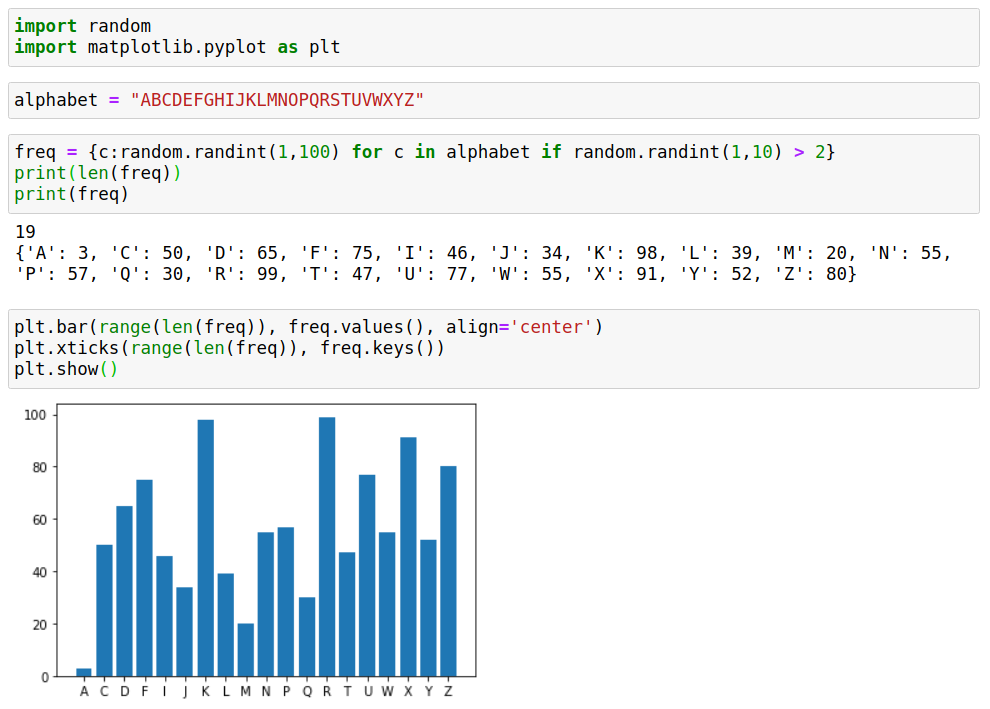
\includegraphics[width=0.9\textwidth]{plot.png}


\end{aufgabe}
% Hier könnt ihr eure Lösung hinschreiben
\begin{loesung} 

\end{loesung}
\newpage
%-----------------------------
\begin{aufgabe}[Substitution \score{20}]
\medskip
Der Schlüsselraum einer Verschlüsselungsfunktion ist die Menge aller
möglichen Schlüssel.

Für eine (allgemeine) \textbf{bijektive} Substitution $s : \Sigma \times K \rightarrow \Sigma$ ist der Schlüsselraum $K$ die Anzahl der möglichen Permutationen des Alphabets
$\Sigma$.

\medskip
\underline{Beispiel}

Sei $\Sigma = \{A,B,C,D\}$ und $(D,C,B,A)$
ein Element des Schlüsselraums, dann gilt 
\begin{align*}
s\Bigl( x, (D,C,B,A) \Bigr) = 
\begin{cases}
D &\mbox{für } x = A \\
C &\mbox{für } x = B \\
B &\mbox{für } x = C \\
A &\mbox{für } x = D 
\end{cases}
\end{align*}

Ein Schlüssel $k$ ist fixpunktfrei, wenn gilt $s_k(x) \not= x$
für alle $x \in \Sigma$. Der Schlüsselraum einer 
fixpunktfreien Substitution enthält nur fixpunktfreie Schlüssel.

\underline{Beispiel}

Für die Caesar-Verschlüsselung sind, bis auf $Z$, alle Schlüssel 
fixpunktfrei.

\smallskip
Ein Schlüssel $k$ ist involutorisch (selbstinverse) wenn gilt
$s\bigl(s(x,k),k\bigr)=x$. Der Schlüsselraum einer 
involutorischen Substitution enthält nur involutorische Schlüssel.

\underline{Beispiel}

Die Caesar-Verschlüsselung mit Schlüsselraum $\{M\}$ ist involutorisch,
dieser Spezialfall ist die ROT13-Verschlüsselung.

\begin{enumerate}
\item 
Bestimmen Sie die Größe des Schlüsselraums $K$ der (allgemeinen) 
Substitution $s : \Sigma \times K \rightarrow \Sigma$
für das Alphabet der Großbuchstaben $\Sigma = \{A, \ldots Z\}$.

Der genaue Wert $x$ muss nicht angegeben werden, aber die Größenordnung
$10^n < x < 10^{n-1}$. \\
\score{4}

\item
Sei $\Sigma = \{00, 01, 10, 11\}$. 
Bestimmen Sie den maximalen Schlüsselraum 
der Substitution $s : \Sigma \times K \rightarrow \Sigma$, wenn
folgendes gilt.

\begin{enumerate}
\item $s$ ist fixpunktfrei\\
\score{8}
\item $s$ ist fixpunktfrei und involutorisch \\
\score{8}
\end{enumerate}

\underline{Hinweis.} Es müssen die Schlüssel, nicht die Größe des
Schlüsselraums angegeben werden.

\end{enumerate}

\underline{Bemerkung}

\smallskip
Die im 2. Weltkrieg eingesetzte Verschlüsselungsmaschine ENIGMA
benutzte konstruktionsbedingt einen involutorischen und fixpunktfreien 
Schlüsselraum. Das war eine der größten Schwächen dieser Verschlüsselung.


\score{20}

\end{aufgabe}
\begin{loesung}

\end{loesung}

\end{document}
